\documentclass{beamer}
\usepackage{graphicx}
\usepackage{listings}
\usetheme{Madrid}

\title{End-to-End Quantum Correlated Imaging Reconstruction with UNet}
\author{Yiwen Tang, Yufan Yao}
\date{May 2025}

\begin{document}

% Title Page
\frame{\titlepage}

% Project Introduction
\begin{frame}{Project Introduction}
\begin{itemize}
    \item This project implements an end-to-end quantum correlated imaging (Ghost Imaging) reconstruction system based on UNet.
    \item Supports multi-frame signal/idler image stacking as multi-channel input, adapted to UNet.
    \item Flexible loss function combination (SSIM, MSE, perceptual loss, etc.), supports weighted loss.
    \item Automated experiment logging and hyperparameter search for easy comparison and reproducibility.
\end{itemize}
\end{frame}

% Data Structure
\begin{frame}{Data Structure and Preprocessing}
\textbf{Each sample directory:}
\begin{itemize}
  \item \texttt{object\_dir/}
  \begin{itemize}
    \item \texttt{signal/} \hspace{1em} \% multi-frame signal images
    \item \texttt{idler/} \hspace{1em} \% multi-frame idler images
    \item \texttt{target.JPG}
  \end{itemize}
\end{itemize}
\vspace{0.5em}
\textbf{Multi-frame stacking and merging:}
\begin{itemize}
    \item Take the first max\_signal/max\_idler signal/idler images
    \item Every stack\_num images are averaged to form one channel
    \item Final input channels: $(\text{max\_signal}//\text{stack\_num}) + (\text{max\_idler}//\text{stack\_num})$
\end{itemize}
\end{frame}

% Data Flow
\begin{frame}{Data Flow and Input Example}
\begin{columns}
\column{0.5\textwidth}

\includegraphics[width=0.95\linewidth]{target_0.png}
\centering {\small Target Example}
\column{0.5\textwidth}
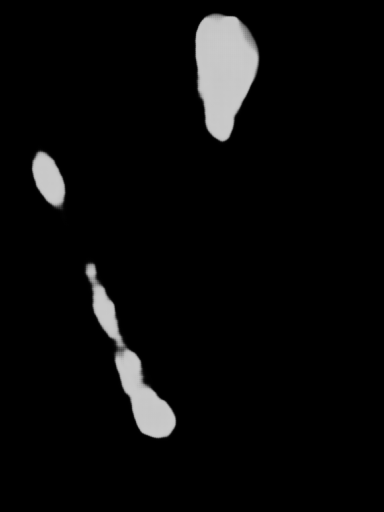
\includegraphics[width=0.95\linewidth]{pred_0.png}
\centering {\small Prediction Example}
\end{columns}
\vspace{0.5em}
\textbf{Input tensor structure:}
\begin{itemize}
    \item $X$: [C, H, W], C is the stacked channel number
    \item target: [1, H, W]
\end{itemize}
\end{frame}

% Model Architecture
\begin{frame}{Model Architecture -- UNet}
\begin{itemize}
    \item Standard UNet structure, supports custom in\_channels for multi-channel input
    \item Symmetric encoder-decoder with skip connections
    \item Output is single-channel reconstructed image
\end{itemize}
\begin{center}
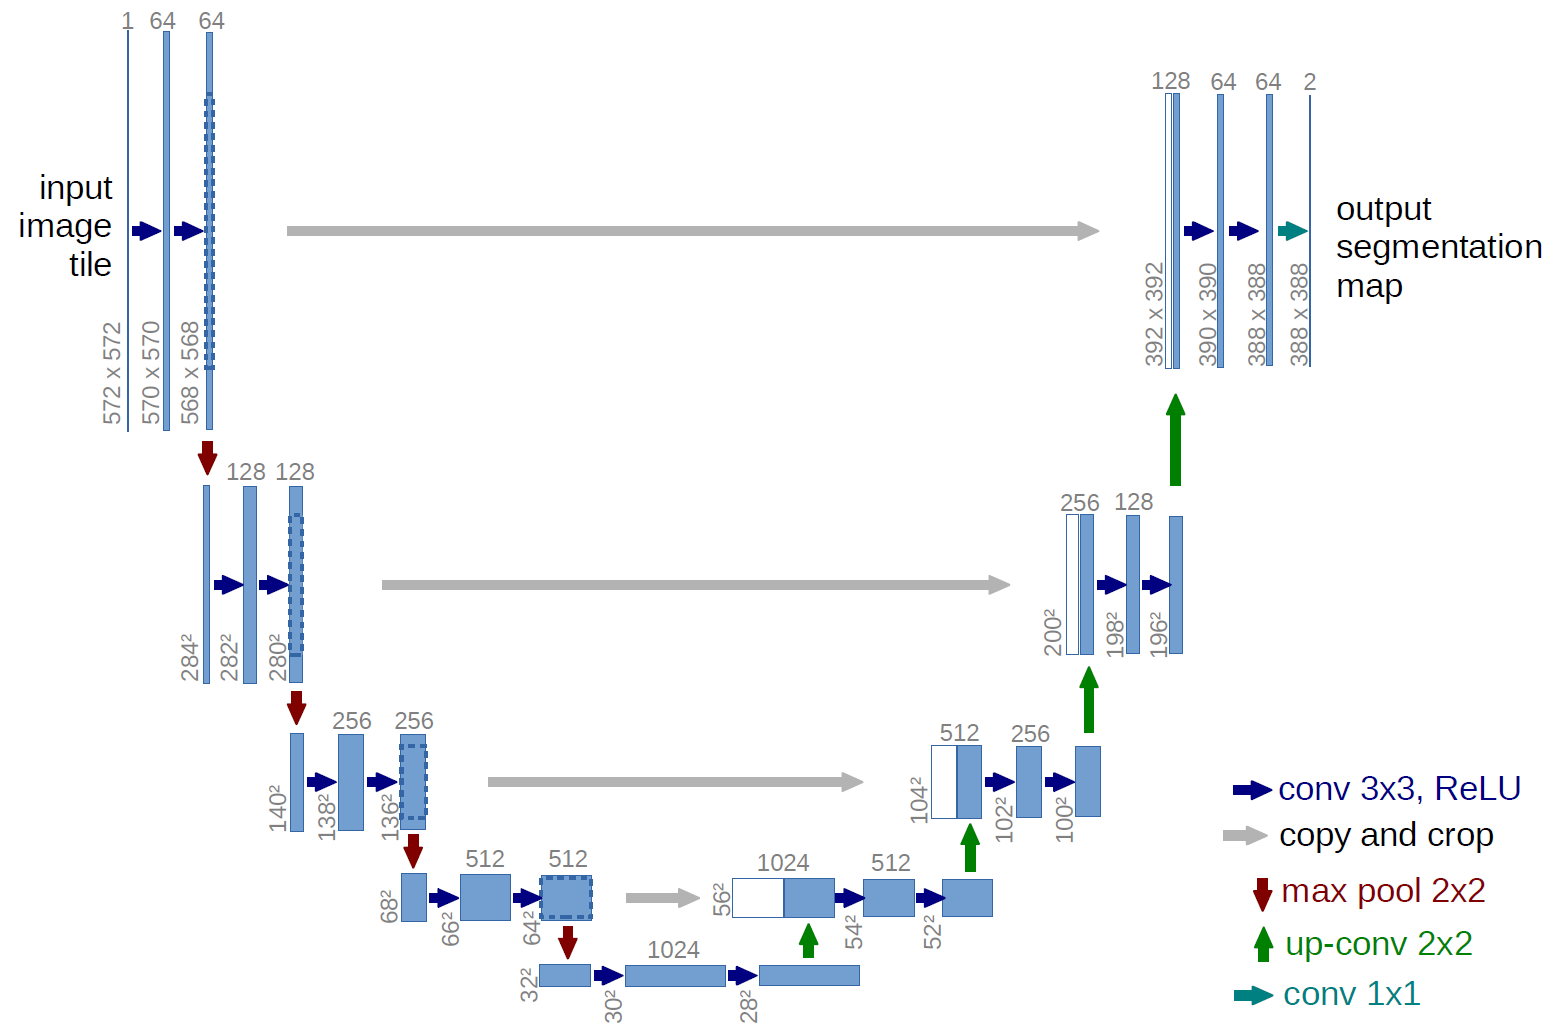
\includegraphics[width=0.8\linewidth]{u-net-architecture.png}
\end{center}
\textit{(To customize, edit model.py)}
\end{frame}

% Loss Function and Training
\begin{frame}{Loss Function and Training}
\textbf{Example loss function:}
\begin{itemize}
    \item \texttt{def loss\_fn(output, target):}
    \item \texttt{\hspace{1em} return w\_ssim * (1 - ssim(output, target))}
    \item \texttt{\hspace{2em} + w\_mse * MSELoss(output, target)}
    \item \texttt{\hspace{2em} + w\_perc * perceptual\_loss(output, target)}
\end{itemize}
\vspace{0.5em}
\begin{itemize}
    \item Supports SSIM, MSE, perceptual loss (VGG16), and weighted combination
    \item Automatically saves best model, loss/PSNR curves, etc.
    \item Each experiment is archived for comparison
\end{itemize}
\end{frame}

% Hyperparameter Search and Logging
\begin{frame}{Hyperparameter Search and Experiment Logging}
\textbf{Optuna search example:}
\begin{itemize}
    \item \texttt{study = optuna.create\_study(direction='minimize')}
    \item \texttt{study.optimize(objective, n\_trials=20)}
\end{itemize}
\vspace{0.5em}
\begin{itemize}
    \item Supports Optuna automated hyperparameter search: stack\_num, learning\_rate, max\_signal, loss weights, etc.
    \item All trial results and best params are logged
    \item Each run generates a unique experiment name, all results archived in results/exp\_xxx/
    \item Each experiment saves:
    \begin{itemize}
        \item Training/validation loss curves (losses.png)
        \item PSNR curve (psnrs.png)
        \item Main hyperparameters and metrics (config.json, metrics.json)
        \item Best model weights (model.pth)
        \item Typical predictions (pred\_*.png, target\_*.png)
    \end{itemize}
    \item File names include main parameters (e.g. exp\_20250531\_003234\_epochs50\_stack2\_lr0.00419\_sig50)
    \item Can automatically extract latest experiment results for evaluation
\end{itemize}
\end{frame}

% Visualization and Examples
\begin{frame}{Visualization and Example Outputs}
\begin{columns}
    \column{0.5\textwidth}
    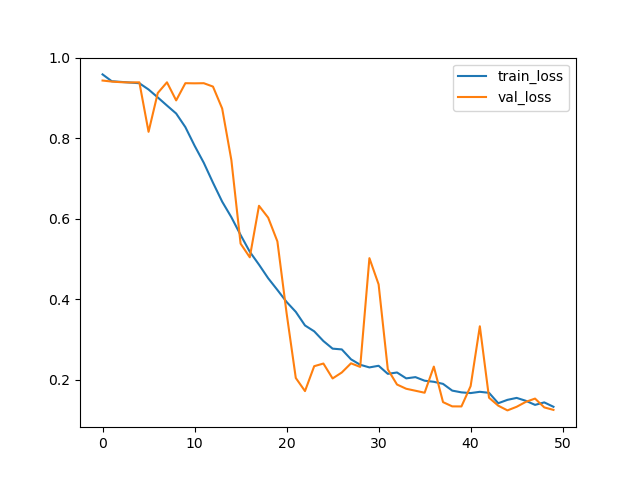
\includegraphics[width=0.95\linewidth]{../results/losses.png}
    \centering {\small Loss Curve}
    \vspace{1em}
    \column{0.5\textwidth}
    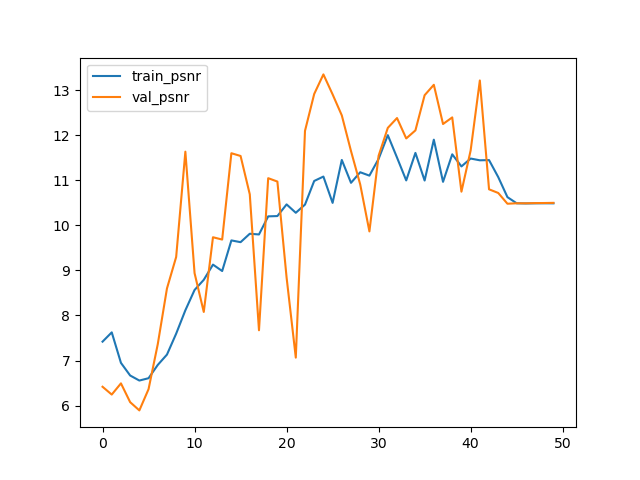
\includegraphics[width=0.95\linewidth]{../results/psnrs.png}
    \centering {\small PSNR Curve (example)}
\end{columns}
\vspace{0.5em}
\begin{itemize}
    \item See previous page for prediction vs. target
    \item More examples in results/ directory
\end{itemize}
\end{frame}

% Main Parameters and Tuning
\begin{frame}{Main Parameters and Tuning}
\begin{itemize}
    \item Tune stack\_num, max\_signal, loss weights manually first, then use Optuna for fine-tuning
    \item PSNR/SSIM are for evaluation, not recommended as loss
    \item Code is modular for easy customization (loss, model, data, etc.)
\end{itemize}
\end{frame}

% PSNR Explanation
\begin{frame}{PSNR Metric Explanation}
    \textbf{PSNR (Peak Signal-to-Noise Ratio)} is a common metric for image reconstruction quality, in dB.
    \begin{itemize}
        \item \textbf{Definition:} $\mathrm{PSNR} = 10 \log_{10}(\mathrm{MAX}^2 / \mathrm{MSE})$
        \item \textbf{MAX} is pixel max (e.g. 1.0 or 255), MSE is mean squared error
        \item \textbf{Range:} Theoretical $[0, +\infty)$, practical $10\sim40$ dB
        \item \textbf{Typical intervals:}
        \begin{itemize}
            \item $<20$ dB: visible distortion
            \item $20\sim30$ dB: acceptable
            \item $30\sim40$ dB: high quality
            \item $>40$ dB: nearly perfect
        \end{itemize}
        \item Higher PSNR means better reconstruction
        \item All PSNR in this project are for [0,1] normalized grayscale images
    \end{itemize}
\end{frame}

% Inference Time Comparison
\begin{frame}{Inference Time Comparison}
\begin{itemize}
    \item \textbf{UNet-based end-to-end model:} ~0.5 seconds per image (on GPU)
    \item \textbf{Traditional ghost imaging reconstruction:} 5--10 minutes per image (CPU, iterative algorithms)
    \item \textbf{Speedup:} 600x--1200x faster
    \item Deep learning enables real-time or near real-time quantum imaging, making practical applications feasible.
\end{itemize}
\end{frame}

% Method Comparison
\begin{frame}{Method Comparison: PSNR and Inference Time}
\begin{table}[]
    \centering
    \begin{tabular}{lcc}
        \hline
        \textbf{Method} & \textbf{PSNR (dB)} & \textbf{Time per Image} \\
        \hline
        Direct Stacking & $\sim$15--20 & $<0.1$ s (GPU/CPU) \\
        UNet (Ours)     & $\sim$28--35 & $\sim$0.5 s (GPU) \\
        Traditional Ghost Imaging & $\sim$20--28 & 5--10 min (CPU) \\
        \hline
    \end{tabular}
    \caption{Comparison of three methods on PSNR and inference/compute time.}
\end{table}
\vspace{0.5em}
\begin{itemize}
    \item UNet achieves the best quality and is orders of magnitude faster than traditional algorithms.
    \item Direct stacking is fast but with poor quality; traditional methods are slow and moderate in quality.
\end{itemize}
\end{frame}

% Conclusion
\begin{frame}{Conclusion}
\begin{itemize}
    \item End-to-end quantum correlated imaging reconstruction, auto experiment logging and hyperparameter search implemented
    \item Welcome to discuss and contribute, see README.md
\end{itemize}
\end{frame}



\end{document}
